\subsection{RecConvSiameseNet}\label{subsec:recconvsnet}
Let us now go into a detailed description of the neural network architecture used in the performed experiments.

\paragraph{Branches}
The proposed architecture (Figure \vref{fig:full_architecture}), named RecConvSiameseNet, involves two information processing branches:
\begin{itemize}
	\item one characterized by LSTM recurrent layers (Rec);
	\item the other featuring several 1D convolutional blocks (Conv), each containing a set of increasing 1D convolutional filters, a batch normalization layer and a 1D average pooling layer, followed by a final dense layer which flattens the feature maps extracted by the convolutional blocks.
\end{itemize}
These two branches receive as input two different types of audio features, extracted upstream during preprocessing, which are respectively:
\begin{itemize}
	\item the more refined $(243 \times 39)$ frames containing MFCCs \& deltas;
	\item the coarsest log-scaled Mel spectrum features contained in $(243 \times 128)$ frames.
\end{itemize}

The "Siamese" part in the name refers to the non-sequential nature of the network, which is typical of Siamese networks \cite{siamesenn}, although the proposed architecture does not have the usual characteristics of Siamese networks, the two branches being completely different from each other.

The basic idea, as mentioned earlier, is to combine the features that these two types of layers are capable to extract, in particular:

\begin{itemize}
	\item LSTM branch being fed with MFCCs \& deltas one $(1 \times 39)$ frame at time, and processing them in the same way, it is able to extract temporal-wise features from the cepstrum, capturing short-term and long-term relationship between frames;
	
	\item convolutional branch being fed with the $(243 \times 128)$ log-scaled Mel spectrum features in their entirety, it is capable of excerpting high-level features that span the entire audio.
\end{itemize}

\begin{figure}
	\centering
	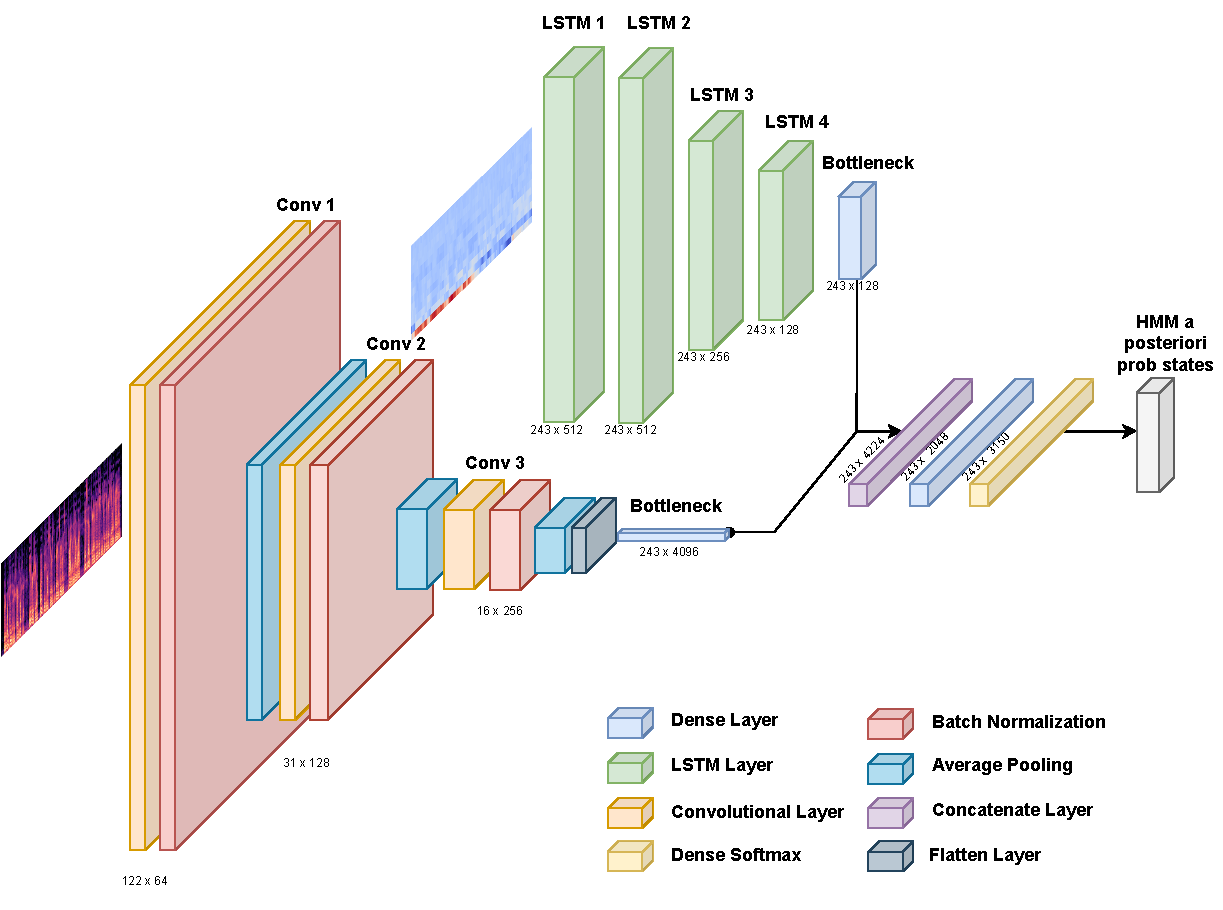
\includegraphics[width=0.5\textwidth]{images/full_architecture}
	\caption{DNN-HMM Architecture}
	\label{fig:full_architecture}
\end{figure}
Further details on architecture and implementation of the two branches will be provided in the sections \vref{subsec:cnnautoencoder} and \vref{subsec:recautoencoder}, where the autoencoder models used during the pre-training phase will be described, as the two RecConvSiameseNet branches were extracted from them prior to the training.

\paragraph{Network tail}
As shown in the Figure \vref{fig:full_architecture}, after the feature extraction process done by the the two branches is completed, the LSTM branch result vector $u_t$ is, at each timestep $t$, concatenated with the flattened feature maps extracted by the convolutional branch $v$ (through repeat vector and concatenation layers), resulting in a new feature vector $w_t = [u_t | v]$. This feature vector is fed into a single network tail, composing of two time-distributed dense layers.

The first one has $\nspeakers \cdot \statesspeakers = 5040$ neuron units, and uses units Leaky ReLU activation function \cite{leakyrelu}, with $\alpha = 0.1$:

$$
\leakyrelu(x) := 
\begin{cases}
	x, & x \geq 0 \\
	\alpha x, & x < 0
\end{cases}
$$
The second one has $\nspeakers \cdot \statesspeakers = 5040$ neuron units too, but since it's the final output layer, it aims to predict the posterior probabilities $P(s_t = k \, | \, o_t)$ of each HMM state $k$ given the current frame $o_t$, and thus uses the softmax activation function (like the one we described in previous section \vref{subsec:dnn}).

Denoting with $W_0, b_0$ and $W_1, b_1$ the weights and biases of the first and second tail dense layers, respectively, the network output on each state can be expressed as:

$$P(s_t = k \, | \, o_t) = \sigma(a_t^T \cdot W_1 + b_1)_k \text{, where: }$$

$$a_t = \leakyrelu(w^T \cdot W_0 + b_0)$$
Details about RecConvSiameseNet training procedure and will be described in section \vref{subsec:recconvsnet_train}, while the architecture of the tail can be seen in Table \vref{tab:tail_recconvsnet}.

\begin{footnotesize}
	\begin{table}
		\centering
		\caption{Parameters of RecConvSiameseNet tail}
		\label{tab:tail_recconvsnet}
		\begin{tabularx}{0.5\textwidth}{XXr}%lMr
			\toprule
			\textbf{Layer Type} & \textbf{Parameters}                                                                   & \textbf{Shape}    \\
			\midrule
			Concatenate layer 	&  																						& (1, 243, 4.224) \\
			Dense               & 				                                                                        & (1, 243, 5040) \\[0.25cm]
			LeakyReLU			&																						& (1, 243, 5040) \\
			Dense				&   																					& (1, 243, 5040) \\
			Softmax				&																						& (1, 243, 5040) \\
			\bottomrule
		\end{tabularx}
		
	\end{table}
	
\end{footnotesize}

